
From the given information, 
\begin{align}
    a^2 &= (\vec{B} - \vec{C})^T(\vec{B} - \vec{C}) \\
    &= 34\\
    c^2 &= (\vec{A} - \vec{B})^T(\vec{A} - \vec{B}) \\
    &= 17\\
    b^2 &= (\vec{C} - \vec{A})^T(\vec{C} - \vec{A}) \\
    &= 17\\
    \implies AB = AC
\end{align}
Thus, the required distance is AD where
\begin{align}
     \vec{D}= \frac{\vec{B} + \vec{C}}{2} = \myvec{\frac{-1}{2}\\ \frac{-1}{2}}
\end{align}
\begin{figure}[htp]
    \centering
    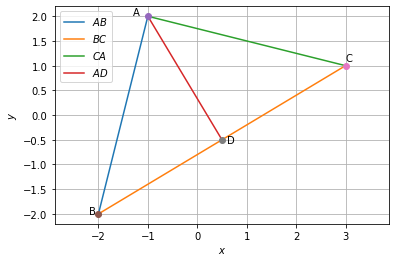
\includegraphics[width=\columnwidth]{solutions/1/1/7/figure/Assignment_1.png}
    \caption{plot}
    \label{rams/1/1/7/fig:my_label}
\end{figure}
and 
\begin{align}
    AD &= \norm{\vec{A} - \vec{D}} \\    
    &= \frac{\sqrt{34}}{2}
\end{align}


